\documentclass[12pt, a4paper]{article}

% --- Cấu hình Tiếng Việt & Font chữ cho pdfLaTeX ---
\usepackage[utf8]{inputenc}
\usepackage[T5]{fontenc}
\usepackage[vietnamese]{babel}
\usepackage{lmodern}

\usepackage{float}
\usepackage[margin=2.5cm]{geometry}
\usepackage{graphicx}
\usepackage{xcolor}
\usepackage{tcolorbox}
\tcbuselibrary{skins, breakable}
\usepackage{fancyvrb}
\usepackage{hyperref}
\usepackage{tikz}

\usetikzlibrary{shapes.geometric, arrows.meta, positioning, calc}

% --- Đường dẫn chứa ảnh ---
\graphicspath{{./log_images/}{./waveform_images/}}

% --- Khai báo màu sắc & Khung ---
\definecolor{codebg}{rgb}{0.96,0.96,0.96}
\definecolor{codeframe}{rgb}{0.8,0.8,0.8}
\definecolor{noteBlue}{rgb}{0.0, 0.45, 0.73}
\definecolor{mainTitle}{rgb}{0.1, 0.2, 0.5}
\definecolor{bugHeaderBg}{rgb}{0.92, 0.94, 0.97}

\newtcolorbox{codebox}{
    colback=codebg,
    colframe=codeframe,
    arc=3pt,
    boxrule=0.8pt,
    left=8pt, right=8pt, top=6pt, bottom=6pt
}

\begin{document}

% =========================================================
%                         TRANG BÌA
% =========================================================
\begin{titlepage}
    \begin{tcolorbox}[
        enhanced,
        colback=white,
        colframe=mainTitle,
        arc=0mm,
        boxrule=1.5pt,
        top=1.5cm, bottom=1.5cm, left=1cm, right=1cm,
        height=\textheight
    ]
        \centering
        
        % Tên Dự Án
        {\Large \bfseries SYNCHRONOUS FIFO VERIFICATION}\\[0.3cm]
        {\large SystemVerilog Verification Environment}\\[2cm]
        
        \rule{0.8\linewidth}{0.8pt}\\[1.5cm]
        
        % Tiêu đề chính của Log Book
        {\Huge \bfseries \color{mainTitle} VERIFICATION DIARY}\\[0.5cm]
        {\Large \bfseries \& DEBUG LOGBOOK}\\[1.5cm]
        
        \rule{0.8\linewidth}{0.8pt}\\[2.5cm]
        
        % Thông tin quản lý Project
        \vfill
        \begin{tabular}{ll}
            \textbf{Project Name:} & Synchronous FIFO Verification \\
            \textbf{Document Type:}& Verification Debug Diary / Bug Tracker \\
            \textbf{Author:}       & Trần Hoàng An \\
            \textbf{Repository:}   & \texttt{synchronous-fifo-verification} \\
        \end{tabular}
        
    \end{tcolorbox}
\end{titlepage}

\newpage
% =========================================================
%                NỘI DUNG LOG ENTRY 01
% =========================================================

\section*{LOG ENTRY \#01: Scoreboard Sampling Read Output Issue}

\begin{tcolorbox}[
    colback=bugHeaderBg,
    colframe=mainTitle,
    arc=2pt,
    boxrule=1pt,
    title=\textbf{ISSUE METADATA \& TRACKING INFO}
]
\begin{tabular}{ll}
    \textbf{Date Logged:}   & 22/07/2026 \\
    \textbf{Issue ID:}      & BUG-20260722-01 \\
    \textbf{Component:}     & Testbench / Mini Scoreboard (\texttt{queue\_test.sv}) \\
    \textbf{Severity:}      & Major (Simulation Failure / False Mismatch) \\
    \textbf{Status:}        & Resolved (Workaround Applied) \\
\end{tabular}
\end{tcolorbox}

\vspace{0.3cm}

\subsection*{Bối cảnh}
Môi trường verification sử dụng monitor để quan sát các giao dịch đọc và ghi của FIFO. Sau đó, monitor tạo đối tượng \texttt{fifo\_transaction} và gửi transaction đến scoreboard thông qua mailbox. Khi có một giao dịch đọc hợp lệ, scoreboard lấy dữ liệu mong đợi từ reference queue rồi so sánh với giá trị \texttt{dout} của DUT.

\subsection*{Hiện tượng}

Khi kiểm tra FIFO bằng reference queue, scoreboard báo lỗi:

\begin{figure}[H]
    \centering
    \fbox{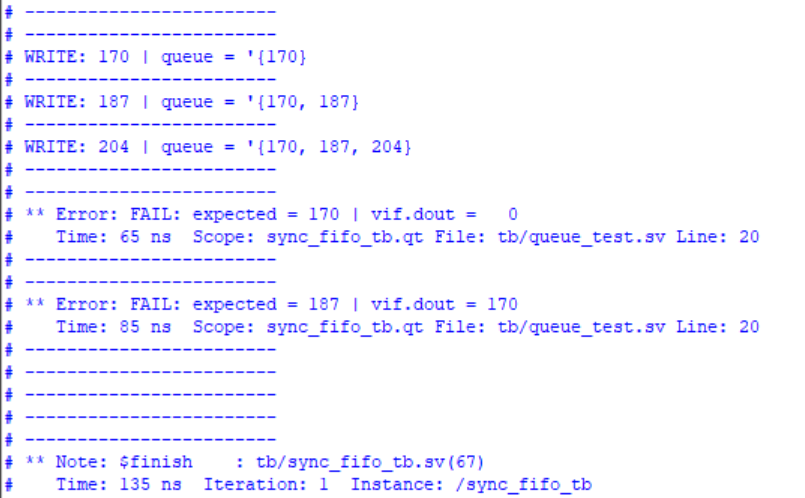
\includegraphics[width=1\linewidth]{console_01.png}} 
    \caption{Ảnh chụp Console Log báo lỗi (Expected vs Actual lệch nhau).}
    \label{fig:console_log}
\end{figure}

Trong khi waveform cho thấy FIFO thực tế vẫn xuất dữ liệu đúng thứ tự:

\begin{codebox}
\begin{verbatim}
170 -> 187 -> ...
\end{verbatim}
\end{codebox}

\begin{figure}[H]
    \centering
    \fbox{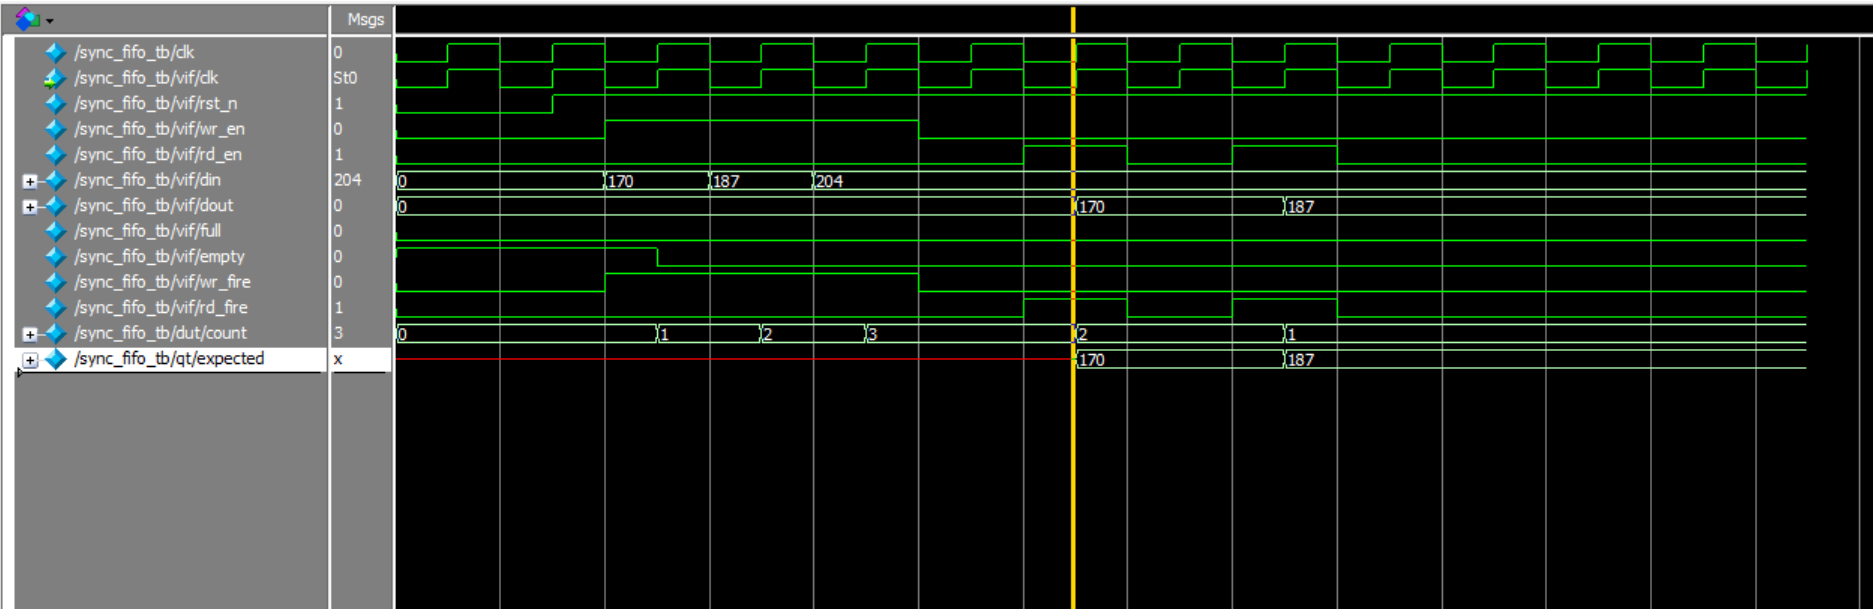
\includegraphics[width=1\linewidth]{waveform_01.png}} 
    \caption{Ảnh chụp Waveform cho thấy FIFO thực tế xuất dữ liệu đúng thứ tự.}
    \label{fig:waveform_01}
\end{figure}

Có thể nhận thấy rằng \texttt{dout} luôn chậm hơn \texttt{expected} một lần đọc (ví dụ Expected: \texttt{BB}, Actual: \texttt{AA}).

\subsection*{Nguyên nhân}

Checker được viết theo dạng:

\begin{codebox}
\begin{verbatim}
always @(posedge vif.clk) begin
    if (vif.rd_fire) begin
        expected = ref_queue.pop_front();

        if (expected !== vif.dout)
            $error(...);
    end
end
\end{verbatim}
\end{codebox}

Trong DUT, \texttt{dout} được cập nhật bằng nonblocking assignment:

\begin{codebox}
\begin{verbatim}
always_ff @(posedge clk or negedge rst_n) begin
    if (!rst_n)
        dout <= '0;
    else if (rd_en && !empty)
        dout <= mem[rd_ptr];
end
\end{verbatim}
\end{codebox}

Tại cùng một cạnh lên của clock, monitor/checker đọc giá trị \texttt{dout} trước khi nonblocking assignment của DUT cập nhật giá trị mới ở vùng NBA region.

Trình tự xảy ra có thể hiểu như sau:

\begin{codebox}
\begin{verbatim}
posedge clk
    |
    +-- Monitor/Checker đọc dout cũ (Active Region)
    |
    +-- DUT thực hiện: dout <= mem[rd_ptr]
    |
    +-- Cuối time step, dout mới được cập nhật (NBA Region)
\end{verbatim}
\end{codebox}

Do đó:

\begin{codebox}
\begin{verbatim}
READ 1:
expected = 170
dout     = 0      // giá trị cũ

READ 2:
expected = 187
dout     = 170    // kết quả của READ trước
\end{verbatim}
\end{codebox}

\begin{figure}[H]
\centering
\begin{tikzpicture}[node distance=1.5cm, >=Stealth, font=\sffamily\small]
    \draw[thick, ->] (0,0) -- (11,0) node[right] {SystemVerilog Region Timeline};
    \draw[thick] (1, 0.15) -- (1, -0.15) node[below] {\texttt{posedge clk}};
    \draw[thick] (4, 0.15) -- (4, -0.15) node[below] {Active Region};
    \draw[thick] (8, 0.15) -- (8, -0.15) node[below] {NBA Region};

    \node[draw, rectangle, rounded corners, fill=red!10, align=center] (mon) at (4, 1.3) {Monitor samples \texttt{dout}\\(Lấy giá trị CŨ)};
    \node[draw, rectangle, rounded corners, fill=green!10, align=center] (dut) at (8, 1.3) {DUT updates new \texttt{dout}\\(\texttt{dout <= mem[rd\_ptr]})};

    \draw[->, dashed, red, thick] (1, 0.3) |- (mon);
    \draw[->, dashed, blue, thick] (4, 0.3) |- (dut);
\end{tikzpicture}
\caption{Sơ đồ minh họa thứ tự lấy mẫu và cập nhật tín hiệu của SystemVerilog.}
\label{fig:log01_b}
\end{figure}

\subsection*{Quá trình phân tích}
Ban đầu, lỗi được nghi ngờ nằm trong scoreboard hoặc reference queue. Tuy nhiên, reference queue vẫn push và pop đúng thứ tự. Dữ liệu expected chính xác, nhưng trường \texttt{dout} bên trong transaction bị sai ngay từ lúc monitor tạo ra. Điều này khẳng định lỗi không nằm ở phép so sánh mà do thời điểm monitor lấy mẫu signal.

\subsection*{Cách xử lý}

Monitor không lấy mẫu \texttt{dout} ngay tại \texttt{posedge clk}. Sau khi phát hiện \texttt{rd\_fire}, monitor chờ đến \texttt{negedge clk} rồi mới đọc \texttt{dout}. Tại thời điểm này, giá trị gán bằng nonblocking assignment đã hoàn toàn ổn định:

\begin{codebox}
\begin{verbatim}
always @(posedge vif.clk) begin
    if (vif.rd_fire) begin
        @(negedge vif.clk); // Chờ đến negedge để dout đã cập nhật xong ở NBA
        tr.dout = vif.dout;
        mon2scb.put(tr);
    end
end
\end{verbatim}
\end{codebox}

\subsection*{Kết quả sau khi sửa}
Scoreboard nhận đúng dữ liệu của từng giao dịch đọc. Expected và actual không còn bị lệch một chu kỳ. các test case basic write/read và wrap-around đều vượt qua chính xác.

\begin{tcolorbox}[colback=noteBlue!5!white, colframe=noteBlue, title=\textbf{Bài học rút ra}]
Đây không nhất thiết là lỗi của FIFO DUT mà là vấn đề về \textbf{thời điểm sampling dữ liệu trong testbench}.

Khi DUT sử dụng nonblocking assignment, giá trị output mới chỉ được cập nhật sau khi các khối kích hoạt tại cạnh clock hiện tại đã thực thi.

Vì vậy, trong verification cần chú ý:
\begin{itemize}
    \item Thời điểm Driver drive tín hiệu.
    \item Thời điểm DUT sample input.
    \item Thời điểm DUT cập nhật output.
    \item Thời điểm Monitor hoặc Scoreboard sample output.
\end{itemize}
Clocking block và Monitor lấy mẫu tại \texttt{negedge} hoặc thông qua offset giúp kiểm soát thời điểm drive và sample tín hiệu, triệt tiêu hoàn toàn \textbf{sampling timing issue}.
\end{tcolorbox}


\newpage
% =========================================================
%                NỘI DUNG LOG ENTRY 02
% =========================================================

\section*{LOG ENTRY \#02: Compilation Unit \& Compile Order Dependency Error}

\begin{tcolorbox}[
    colback=bugHeaderBg,
    colframe=mainTitle,
    arc=2pt,
    boxrule=1pt,
    title=\textbf{ISSUE METADATA \& TRACKING INFO}
]
\begin{tabular}{ll}
    \textbf{Date Logged:}   & 23/07/2026 \\
    \textbf{Issue ID:}      & BUG-20260723-02 \\
    \textbf{Component:}     & Build Environment / Compilation Scripts \\
    \textbf{Severity:}      & Critical (Compilation \& Elaboration Failure) \\
    \textbf{Status:}        & Resolved \\
\end{tabular}
\end{tcolorbox}

\vspace{0.3cm}

\subsection*{Bối cảnh}
Môi trường verification được chia thành nhiều file riêng biệt: \texttt{fifo\_transaction.sv}, \texttt{fifo\_monitor.sv}, \texttt{fifo\_scoreboard.sv}, \texttt{fifo\_if.sv}, \texttt{sync\_fifo.sv}, và \texttt{fifo\_tb.sv}. Monitor sử dụng class \texttt{fifo\_transaction}. Testbench đồng thời instantiate interface \texttt{fifo\_if} và DUT \texttt{sync\_fifo}.

\subsection*{Hiện tượng}
Trong quá trình compile trên ModelSim xuất hiện nhiều lỗi không tìm thấy class hoặc design unit:

\begin{figure}[H]
    \centering
    \fbox{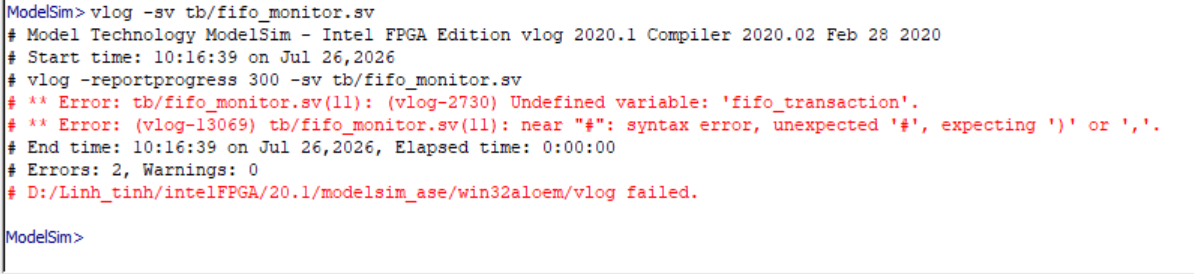
\includegraphics[width=1\linewidth]{console_02_a.png}} 
    \caption{Ảnh console ModelSim hiển thị lỗi \texttt{fifo\_transaction} không được nhận diện.}
    \label{fig:console_02_a}
\end{figure}

\begin{figure}[H]
    \centering
    \fbox{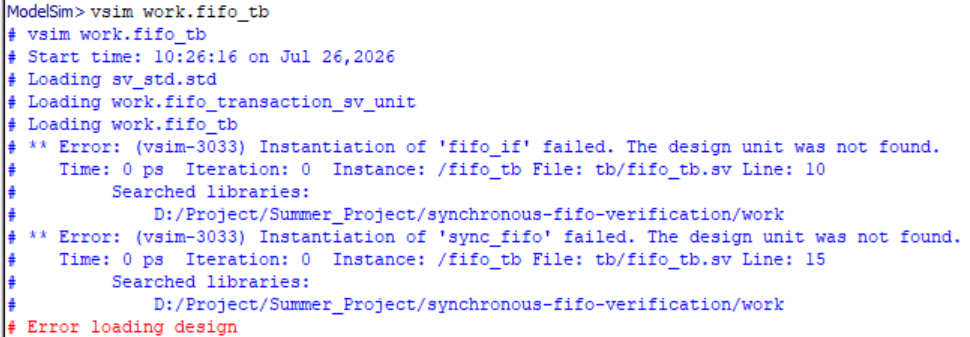
\includegraphics[width=1\linewidth]{console_02_b.png}} 
    \caption{Ảnh console ModelSim hiển thị lỗi không tìm thấy design unit \texttt{fifo\_if} hoặc \texttt{sync\_fifo}.}
    \label{fig:console_02_b}
\end{figure}

Các lỗi tiêu biểu bao gồm:
\begin{codebox}
\begin{verbatim}
Undefined variable or unknown type: fifo_transaction
Instantiation of fifo_if failed. The design unit was not found.
Instantiation of sync_fifo failed. The design unit was not found.
\end{verbatim}
\end{codebox}

\subsection*{Nguyên nhân}
Nguyên nhân chính nằm ở cách các file được compile và khả năng nhìn thấy nhau (visibility) giữa các compilation unit:
\begin{enumerate}
    \item khi \texttt{fifo\_transaction.sv} và \texttt{fifo\_monitor.sv} biên dịch riêng lẻ, ModelSim xem chúng thuộc các compilation unit khác nhau. Vì class không nằm trong \texttt{package}, monitor không thể nhìn thấy định nghĩa class.
    \item \texttt{fifo\_if} và \texttt{sync\_fifo} chưa được compile vào thư viện \texttt{work} trước khi \texttt{fifo\_tb.sv} elaboration.
    \item Tên file trong lệnh compile bị lệch với tên thật (ví dụ lệnh biên dịch tìm \texttt{tb/sync\_fifo\_scoreboard.sv} nhưng file thực tế là \texttt{tb/fifo\_scoreboard.sv}).
\end{enumerate}

\begin{figure}[H]
\centering
\begin{tikzpicture}[node distance=1.8cm, >=Stealth, font=\sffamily\small]
    \node[draw, rectangle, fill=blue!10, rounded corners] (trans) {\texttt{fifo\_transaction.sv}};
    \node[draw, rectangle, fill=blue!10, rounded corners, right=of trans] (mon) {\texttt{fifo\_monitor.sv}};
    \node[draw, rectangle, fill=blue!10, rounded corners, right=of mon] (scb) {\texttt{fifo\_scoreboard.sv}};
    
    \node[draw, rectangle, fill=green!10, rounded corners, below=1cm of trans] (if) {\texttt{fifo\_if.sv}};
    \node[draw, rectangle, fill=green!10, rounded corners, below=1cm of scb] (dut) {\texttt{sync\_fifo.sv}};
    \node[draw, rectangle, fill=red!10, rounded corners, below=1cm of mon] (tb) {\texttt{fifo\_tb.sv}};

    \draw[->, thick] (trans) -- (mon);
    \draw[->, thick] (mon) -- (scb);
    \draw[->, thick] (if) -- (tb);
    \draw[->, thick] (dut) -- (tb);
\end{tikzpicture}
\caption{Sơ đồ phụ thuộc thứ tự biên dịch (File bên trái phải biên dịch trước file bên phải).}
\label{fig:log02_c}
\end{figure}

\subsection*{Quá trình phân tích}
Ban đầu, lỗi nghi ngờ do cú pháp typed mailbox không tương thích. Tuy nhiên, việc kiểm tra thư viện \texttt{work} cho thấy module và interface chưa tồn tại ở thời điểm elaboration. Lỗi hoàn toàn xuất phát từ script build và compilation unit dependency.

\subsection*{Cách khắc phục}
Sử dụng tùy chọn \texttt{-mfcu} (Multi-File Compilation Unit) để compile các file class chung một unit, chuẩn hóa thứ tự biên dịch RTL/Interface trước Testbench, và sửa đường dẫn file:

\begin{codebox}
\begin{verbatim}
vlib work
vlog -sv rtl/sync_fifo.sv
vlog -sv tb/fifo_if.sv
vlog -sv -mfcu tb/fifo_transaction.sv tb/fifo_monitor.sv tb/fifo_scoreboard.sv
vlog -sv tb/fifo_tb.sv
vsim work.fifo_tb
run -all
\end{verbatim}
\end{codebox}

\begin{figure}[H]
    \centering
    \fbox{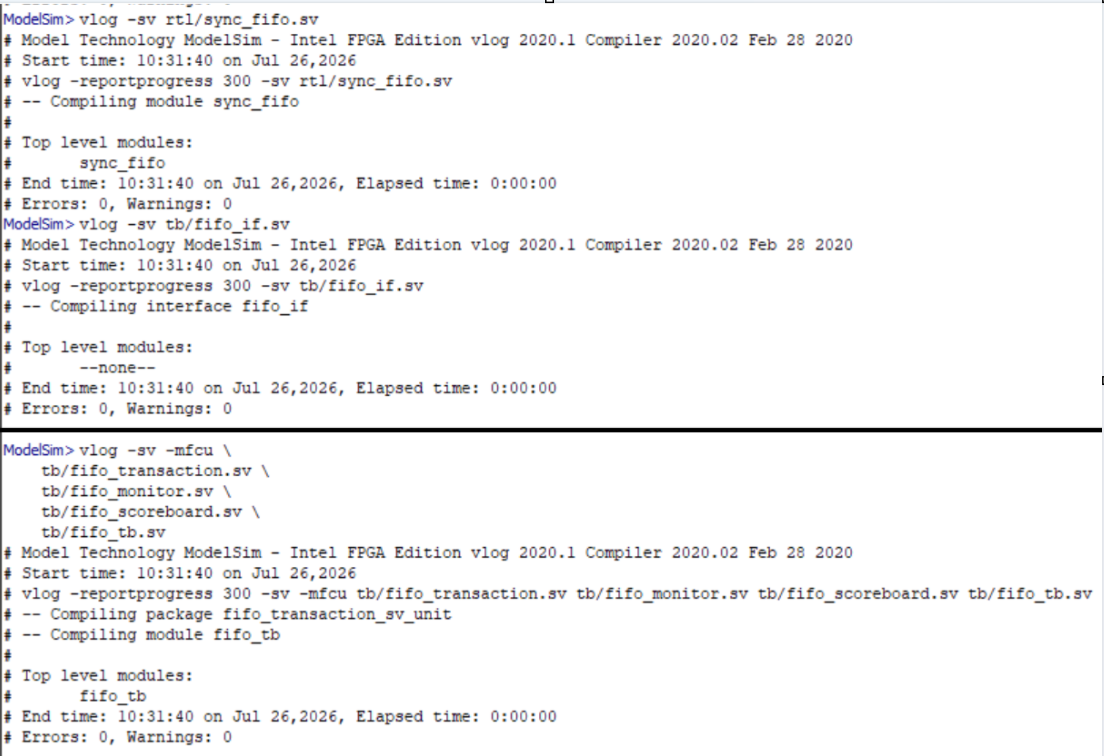
\includegraphics[width=1\linewidth]{console_02_c.png}} 
    \caption{Đoạn lệnh compile đúng thứ tự với tùy chọn -mfcu.}
    \label{fig:console_02_d}
\end{figure}

\subsection*{Kết quả sau khi sửa}
ModelSim nhận diện đầy đủ class, interface và module. Testbench elaboration thành công và mô phỏng bình thường.

\begin{tcolorbox}[colback=noteBlue!5!white, colframe=noteBlue, title=\textbf{Bài học rút ra}]
\begin{itemize}
    \item Thứ tự compile và phạm vi nhìn thấy (scope visibility) của class là yếu tố then chốt trong SystemVerilog.

    \item Việc một file đã compile trước không đồng nghĩa class trong đó tự động nhìn thấy từ compilation unit khác.
\end{itemize}
\end{tcolorbox}


\newpage
% =========================================================
%                NỘI DUNG LOG ENTRY 03
% =========================================================

\section*{LOG ENTRY \#03: Ineffective Scoreboard Delay Fix}

\begin{tcolorbox}[
    colback=bugHeaderBg,
    colframe=mainTitle,
    arc=2pt,
    boxrule=1pt,
    title=\textbf{ISSUE METADATA \& TRACKING INFO}
]
\begin{tabular}{ll}
    \textbf{Date Logged:}   & 24/07/2026 \\
    \textbf{Issue ID:}      & BUG-20260724-03 \\
    \textbf{Component:}     & Scoreboard Architecture / Timing \\
    \textbf{Severity:}      & Medium (Conceptual \& Architectural Error) \\
    \textbf{Status:}        & Resolved \\
\end{tabular}
\end{tcolorbox}

\vspace{0.3cm}

\subsection*{Bối cảnh}
Sau khi phát hiện dữ liệu đọc bị lấy mẫu quá sớm ở Log Entry \#01, một giải pháp ban đầu được thử nghiệm là giữ nguyên Monitor và thêm delay bên trong Scoreboard trước khi so sánh \texttt{actual} và \texttt{expected}.

\subsection*{Hiện tượng}
Dù Scoreboard chờ thêm một khoảng thời gian (\texttt{\#5ns} hoặc \texttt{@(posedge clk)}), giá trị \texttt{actual} vẫn bị sai và không hề thay đổi. Scoreboard vẫn so sánh dữ liệu cũ.


\subsection*{Nguyên nhân}
Transaction là một \textbf{snapshot (ảnh chụp cố định)} của tín hiệu tại thời điểm Monitor thực hiện gán:
\begin{codebox}
\begin{verbatim}
tr.dout = vif.dout;
mon2scb.put(tr);
\end{verbatim}
\end{codebox}
Sau khi \texttt{tr.dout} được gán, dữ liệu nằm trong biến này hoàn toàn độc lập và không hề liên kết với tín hiệu \texttt{vif.dout} trên interface. Việc Scoreboard hoãn xử lý chỉ hoãn thời điểm so sánh chứ không thay đổi được nội dung bức ảnh snapshot đã chụp sai từ trước.

\begin{figure}[H]
\centering
\begin{tikzpicture}[font=\sffamily\small]
    \draw[thick, ->] (0,0) -- (10,0) node[right] {Time};
    
    \node at (2, 0.4) {$T_1$ (Monitor sampling)};
    \node at (7, 0.4) {$T_2$ (Scoreboard delay finished)};
    
    % Interface signal line
    \draw[red, thick] (0,-0.8) -- (3.5,-0.8) node[midway, above]{\texttt{vif.dout = AA}} -- (3.5,-1.6) -- (9.5,-1.6) node[midway, above]{\texttt{vif.dout = BB}};
    \node[left] at (0,-1.2) {Interface \texttt{vif.dout}:};

    % Transaction object value
    \draw[blue, thick, fill=blue!5] (2,-2.5) rectangle (8.5,-3.2);
    \node at (5.25,-2.85) {\textbf{\texttt{tr.dout = AA}} (Static Value inside Transaction)};
    \node[left] at (0,-2.85) {Object \texttt{tr.dout}:};

    \draw[->, dashed, black, thick] (2,-0.9) -- (2,-2.4) node[midway, right] {Copy snapshot};
\end{tikzpicture}
\caption{Minh họa sự khác biệt giữa tín hiệu động trên Interface và dữ liệu tĩnh trong Transaction.}
\label{fig:log03_b}
\end{figure}

\subsection*{Cách khắc phục}
Xóa bỏ toàn bộ delay trong Scoreboard. Thời điểm lấy mẫu phải được sửa triệt để ngay tại Monitor.
\begin{enumerate}
    \item Monitor chờ \texttt{dout} ổn định mới gán \texttt{tr.dout = vif.dout} rồi gửi qua mailbox.
    \item Scoreboard tuân thủ đúng chức năng: Nhận transaction $\rightarrow$ Cập nhật Reference Model $\rightarrow$ So sánh và Report PASS/FAIL.
\end{enumerate}

\subsection*{Kết quả sau khi sửa}
Transaction chứa đúng dữ liệu ngay khi tạo ra. Scoreboard chạy mượt mà không cần thêm bất kỳ lệnh delay nào.

\begin{tcolorbox}[colback=noteBlue!5!white, colframe=noteBlue, title=\textbf{Bài học rút ra}]
Phân định rõ trách nhiệm (Separation of Concerns) trong Layered Testbench:
\begin{itemize}
    \item \textbf{Monitor:} Chịu trách nhiệm hoàn toàn về Timing và lấy mẫu tín hiệu đúng thời điểm.
    \item \textbf{Scoreboard:} Chịu trách nhiệm kiểm tra logic dữ liệu.
    \item Một khi Transaction đã thu thập sai dữ liệu, trì hoãn xử lý ở Scoreboard không thể khôi phục dữ liệu đúng.
\end{itemize}
\end{tcolorbox}


\newpage
% =========================================================
%                NỘI DUNG LOG ENTRY 04
% =========================================================

\section*{LOG ENTRY \#04: Ignored Rejected Operations in Accepted-Only Scoreboard}

\begin{tcolorbox}[
    colback=bugHeaderBg,
    colframe=mainTitle,
    arc=2pt,
    boxrule=1pt,
    title=\textbf{ISSUE METADATA \& TRACKING INFO}
]
\begin{tabular}{ll}
    \textbf{Date Logged:}   & 25/07/2026 \\
    \textbf{Issue ID:}      & BUG-20260725-04 \\
    \textbf{Component:}     & Monitor / Scoreboard / Protocol Checker \\
    \textbf{Severity:}      & Medium (Test Coverage Hole) \\
    \textbf{Status:}        & Resolved \\
\end{tabular}
\end{tcolorbox}

\vspace{0.3cm}

\subsection*{Bối cảnh}
Monitor ban đầu chỉ tạo transaction khi một thao tác thực sự được DUT chấp nhận:
\begin{codebox}
\begin{verbatim}
wr_fire = wr_en && !full;
rd_fire = rd_en && !empty;
\end{verbatim}
\end{codebox}
Monitor chỉ gửi transaction đến scoreboard khi \texttt{wr\_fire} hoặc \texttt{rd\_fire} bằng 1.

\subsection*{Hiện tượng}
Trong test case \textbf{Read when empty}, testbench kích hoạt \texttt{rd\_en = 1} lúc FIFO đang \texttt{empty}. Tương tự với \textbf{Write when full}, kích hoạt \texttt{wr\_en = 1} lúc \texttt{full = 1}. Tối ưu là DUT phải chặn thao tác. Tuy nhiên, Scoreboard hoàn toàn không in bất kỳ thông báo PASS hay FAIL nào cho các sự kiện này.

\begin{figure}[H]
    \centering
    \fbox{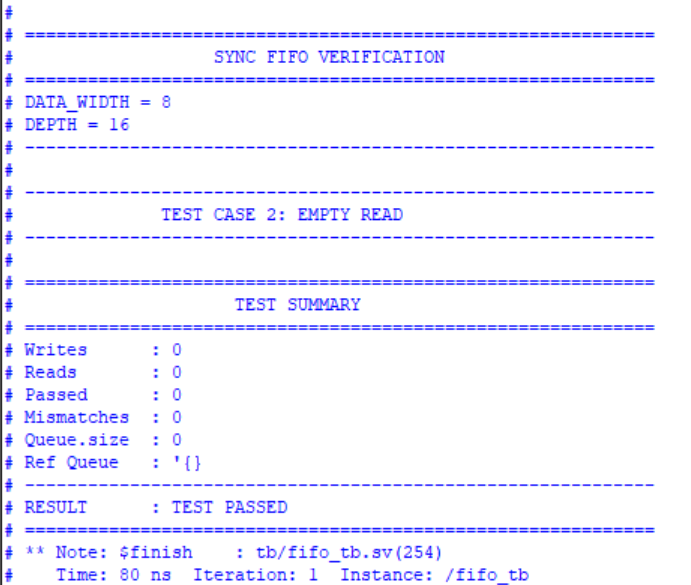
\includegraphics[width=1\linewidth]{console_04_a.png}} 
    \caption{Console log thể hiện testbench có phát request nhưng Monitor không gửi transaction.}
    \label{fig:console_04_a}
\end{figure}

\subsection*{Nguyên nhân}
Khi FIFO empty, \texttt{rd\_fire = 1 \&\& 0 = 0}. Do \texttt{rd\_fire = 0}, Monitor bỏ qua và không tạo transaction gửi qua Mailbox. Scoreboard thụ động chỉ xử lý những gì nhận từ Mailbox nên hoàn toàn "mù" trước ý định kích hoạt yêu cầu của testbench.

\subsection*{Ý nghĩa \& Phân tích}
Scoreboard thông thường được thiết kế để kiểm tra dữ liệu của \textbf{Accepted Transactions}. Các thao tác bị từ chối (\textbf{Rejected Operations}) như *Read when empty* hay *Write when full* thuộc nhóm kiểm tra giao thức (protocol/corner-case checking). Nếu chỉ quan sát \texttt{fire}, testbench sẽ bỏ sót coverage của các góc cấm này.

\subsection*{Cách kiểm tra và xử lý hiện tại}

Ở giai đoạn này, testbench chưa sử dụng SystemVerilog Assertions để tự động kiểm tra thao tác đọc khi FIFO rỗng. Thay vào đó, corner case này được kiểm tra thủ công thông qua stimulus và waveform.

Test case được xây dựng theo trình tự:
\begin{enumerate}
    \item Reset FIFO để đưa hệ thống về trạng thái ban đầu.
    \item Ghi một giá trị \texttt{8'hAA} vào FIFO.
    \item Thực hiện lệnh đọc lần thứ nhất để lấy phần tử \texttt{8'hAA} ra khỏi FIFO.
    \item Thực hiện lệnh đọc lần thứ hai khi FIFO đã rỗng.
    \item Quan sát waveform để xác nhận rằng chỉ lần đọc thứ nhất được chấp nhận, còn lần đọc thứ hai bị FIFO từ chối.
\end{enumerate}

\begin{codebox}
\begin{verbatim}
task automatic tc2_empty_read();
    reset_dut();

    // Ghi mot phan tu vao FIFO
    write_data(8'hAA);

    // Lan doc thu nhat: hop le, doc du lieu AA
    read_data();

    // Lan doc thu hai: FIFO da empty, yeu cau bi tu choi
    read_data();
endtask
\end{verbatim}
\end{codebox}

Trong waveform, lần đọc thứ nhất xảy ra khi \texttt{empty = 0}, do đó điều kiện giao dịch đọc hợp lệ:
\begin{center}
    \texttt{rd\_fire = rd\_en \&\& !empty}
\end{center}
nhận giá trị bằng 1 và dữ liệu \texttt{8'hAA} được đọc ra khỏi FIFO.

Sau lần đọc này, FIFO chuyển sang trạng thái rỗng và tín hiệu \texttt{empty} được đưa lên 1. Khi lệnh \texttt{read\_data()} thứ hai tiếp tục kích hoạt \texttt{rd\_en}, điều kiện \texttt{rd\_fire} vẫn bằng 0 vì \texttt{empty = 1}. Điều đó chứng tỏ DUT không chấp nhận thao tác đọc thứ hai.

\begin{figure}[H]
    \centering
    \fbox{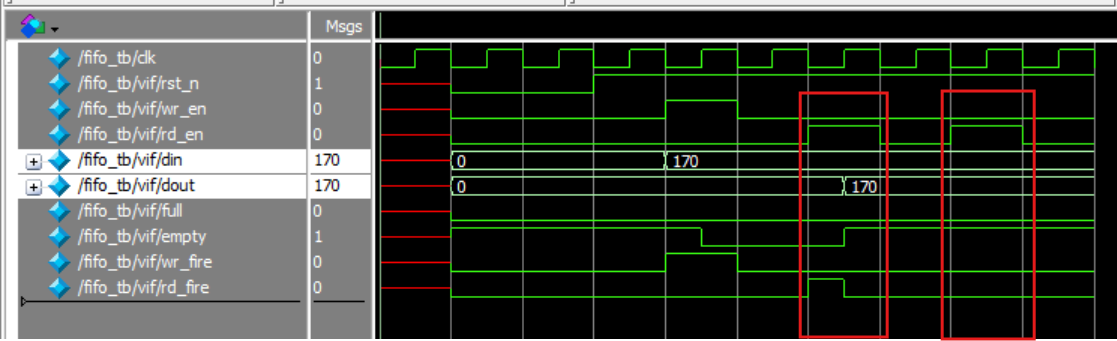
\includegraphics[width=0.95\linewidth]{waveform_04_b.png}}
    \caption{Waveform của test case Empty Read: lần đọc thứ nhất được chấp nhận, trong khi lần đọc thứ hai bị từ chối do FIFO đã rỗng.}
    \label{fig:waveform_empty_read}
\end{figure}

\subsection*{Kết quả kiểm tra}

Waveform cho thấy chỉ có một giao dịch đọc hợp lệ được thực hiện sau khi ghi giá trị \texttt{8'hAA}. Ở yêu cầu đọc tiếp theo, \texttt{rd\_en} được kích hoạt nhưng \texttt{rd\_fire} không được tạo ra vì tín hiệu \texttt{empty} đang ở mức 1.

Kết quả này xác nhận FIFO đã từ chối thao tác đọc khi rỗng đúng với thiết kế. Tuy nhiên, việc kiểm tra hiện tại vẫn phụ thuộc vào quan sát waveform và chưa được tự động hóa bằng Assertion.

% --- Khung Bài học kinh nghiệm đồng bộ với giao diện chung ---
\begin{tcolorbox}[colback=noteBlue!5!white, colframe=noteBlue, title=\textbf{Bài học kinh nghiệm}]
Một test case đọc khi FIFO rỗng cần tạo được rõ ràng cả hai trường hợp: một lần đọc hợp lệ và một lần đọc bị từ chối. 

Việc ghi một phần tử rồi thực hiện hai lần đọc liên tiếp giúp waveform thể hiện trực quan sự khác biệt giữa một giao dịch được chấp nhận và một yêu cầu bị chặn bởi trạng thái \texttt{empty}.
\end{tcolorbox}



\newpage
% =========================================================
%                NỘI DUNG LOG ENTRY 05
% =========================================================

\section*{LOG ENTRY \#05: Simultaneous Read/Write Timing Alignment Issue}

\begin{tcolorbox}[
    colback=bugHeaderBg,
    colframe=mainTitle,
    arc=2pt,
    boxrule=1pt,
    title=\textbf{ISSUE METADATA \& TRACKING INFO}
]
\begin{tabular}{ll}
    \textbf{Date Logged:}   & 26/07/2026 \\
    \textbf{Issue ID:}      & BUG-20260726-05 \\
    \textbf{Component:}     & Stimulus Generator / Sequence Task \\
    \textbf{Severity:}      & Minor (False Positive Test / Insufficient Stimulus) \\
    \textbf{Status:}        & Resolved \\
\end{tabular}
\end{tcolorbox}

\vspace{0.3cm}

\subsection*{Bối cảnh}
Test case \textbf{Simultaneous Read/Write} được tạo ra để kiểm tra khả năng FIFO thực hiện đồng thời một thao tác ghi và một thao tác đọc trong cùng một chu kỳ clock (\texttt{wr\_en = 1} và \texttt{rd\_en = 1} tại cùng \texttt{posedge clk}).

\begin{codebox}
\begin{verbatim}
task automatic tc5_simultaneous_rw(); 
    $display("----------------------------------------"); 
    $display(" TEST CASE 5: Simultaneous READ / WRITE"); 
    $display("----------------------------------------"); 
    reset_dut(); @(negedge vif.clk); 
    write_data(8'hAA); 
    write_data(8'hBB); 
    write_data(8'hCC); 

    @(negedge vif.clk); 
    write_data(8'hDD); 
    read_data(); read_data(); 

    @(negedge vif.clk); 
    write_data(8'hEE); 
    write_data(8'hFF); 

endtask
\end{verbatim}
\end{codebox}

\subsection*{Hiện tượng}
Test case báo PASS, nhưng khi soi Waveform thì thấy \texttt{wr\_en} và \texttt{rd\_en} không hề cùng bằng 1 tại bất kỳ cạnh lên clock nào. Tín hiệu này bật ở chu kỳ trước, bị hạ xuống rồi tín hiệu kia mới bật ở chu kỳ sau.

\begin{figure}[H]
    \centering
    \fbox{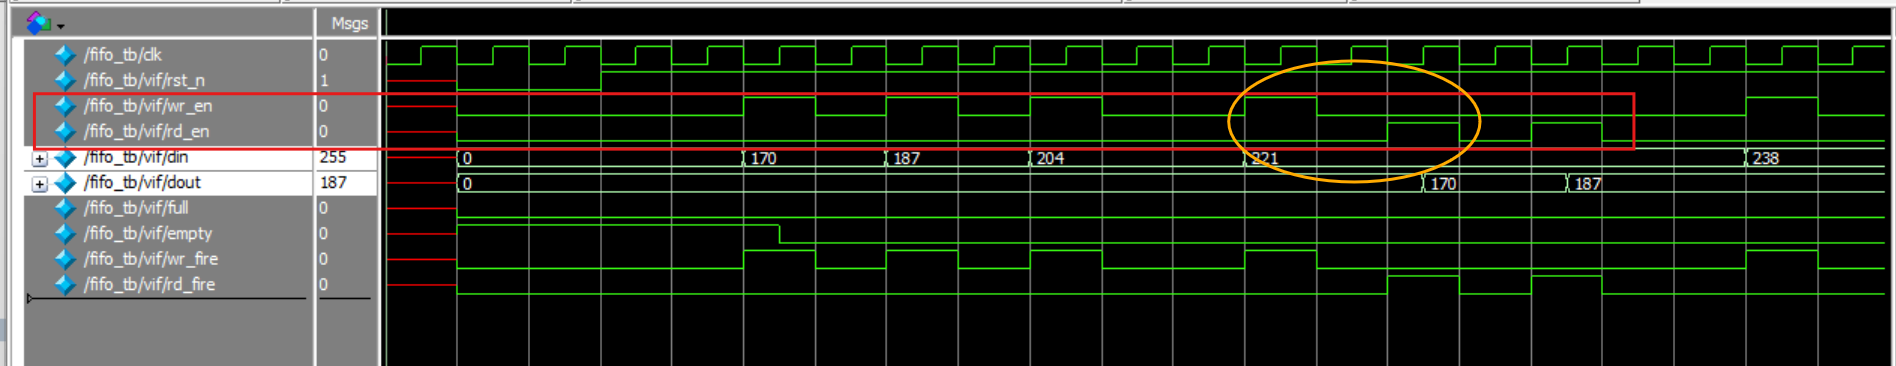
\includegraphics[width=1\linewidth]{waveform_05_a.png}} 
    \caption{Waveform lỗi cho thấy wr\_en và rd\_en bị lệch nhau một chu kỳ.}
    \label{fig:waveform_05_a}
\end{figure}

\subsection*{Nguyên nhân}
Các task \texttt{write\_data()} và \texttt{read\_data()} được thiết kế tuần tự, mỗi task tự quản lý enable và tự chờ cạnh clock:
\begin{codebox}
\begin{verbatim}
write_data(data); // Chờ 1 clock cycle để hoàn thành
read_data();      // Chạy ở clock cycle tiếp theo
\end{verbatim}
\end{codebox}
Khi gọi nối tiếp, thao tác ghi hoàn thành xong mới đến thao tác đọc. Dù dùng \texttt{fork...join}, nếu cơ chế chờ clock bên trong 2 task lệch nhau thì tín hiệu vẫn không trùng khớp tại 1 xung nhịp.

\subsection*{Cách khắc phục}
Điều khiển trực tiếp \texttt{wr\_en} và \texttt{rd\_en} trong cùng một chu kỳ clock, thay vì gọi các task tuần tự. Cụ thể, trong test case, sau khi reset và ghi dữ liệu ban đầu, trực tiếp drive cả hai enable cùng lúc:
\begin{codebox}
\begin{verbatim}
task automatic tc5_simultaneous_rw();
       
        reset_dut();

        @(negedge vif.clk);
        write_data(8'hAA);
        write_data(8'hBB);
        write_data(8'hCC);
        
        // Drive trực tiếp wr_en và rd_en thì mới có xung cùng lúc
        @(negedge vif.clk);         
        vif.din = 8'hDD;
        vif.wr_en = 1;
        vif.rd_en = 1;

        @(negedge vif.clk);
        vif.wr_en = 0;
        vif.rd_en = 0;

        @(negedge vif.clk);
        write_data(8'hDD);
        read_data();

    endtask
\end{verbatim}
\end{codebox}



\begin{figure}[H]
    \centering
    \fbox{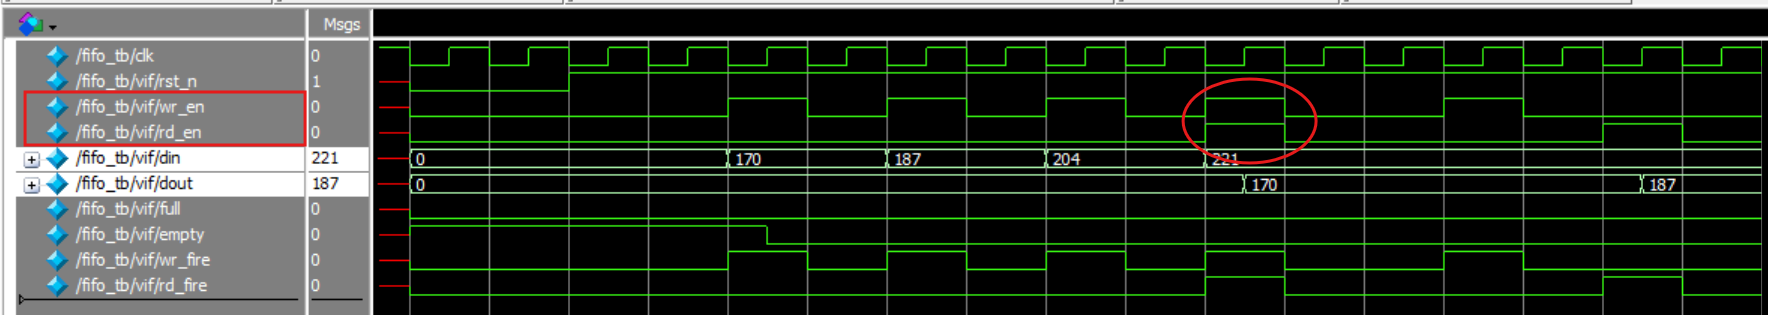
\includegraphics[width=1\linewidth]{waveform_05_b.png}} 
    \caption{Waveform sau khi sửa: wr\_en và rd\_en cùng bằng 1 tại cùng một posedge clk.}
    \label{fig:waveform_05_b}
\end{figure}

\subsection*{Kết quả sau khi sửa}
Monitor ghi nhận cả Write transaction và Read transaction trong cùng 1 chu kỳ. Reference queue vừa pop phần tử cũ vừa push phần tử mới chính xác.

\begin{tcolorbox}[colback=noteBlue!5!white, colframe=noteBlue, title=\textbf{Bài học rút ra}]
Một Test Case báo PASS không có nghĩa là corner case mong muốn đã thực sự được kích hoạt!
\begin{itemize}
    \item Tên task hay tên test case không đảm bảo tín hiệu tạo ra đúng thời điểm.
    \item Luôn luôn đối chiếu sóng Waveform hoặc dùng Assertion để kiểm chứng stimulus đã tạo đúng điều kiện biên (Corner Case) hay chưa.
\end{itemize}
\end{tcolorbox}

\end{document}